
\begin{flushleft}
The python code for the figure is
\begin{lstlisting}
./code/traingle.py
\end{lstlisting}
The latex- tikz code is
\begin{lstlisting}
./figs/triangle.tex
\end{lstlisting}
The above latex code can be compiled as standalone document
\begin{lstlisting}
./figs/triangle_fig.tex
\end{lstlisting}
\end{flushleft}
%\begin{columns}
%\column{0.5\textwidth}
\begin{figure}[H]
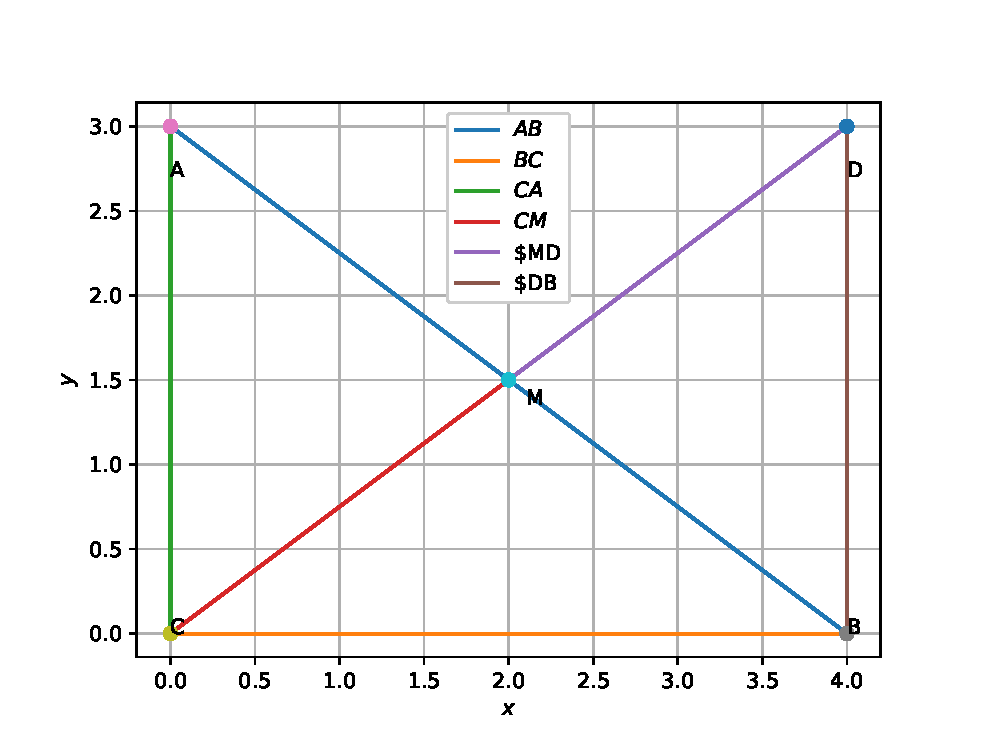
\includegraphics[scale=0.4]{./figs/triangle.eps}
\caption*{a) By Python}
%


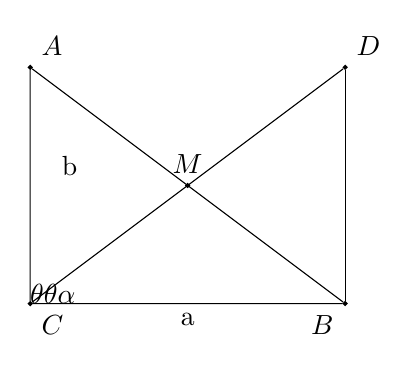
\begin{tikzpicture}
[scale=1,>=stealth,point/.style={draw,circle,fill = black,inner sep=0.5pt},]

%Triangle sides
\def\a{4}
\def\b{3}
\def\c{sqrt(\a^2+\c^2)}



%Labeling points
\node (A) at (0,\b)[point,label=above right:$A$] {};
\node (B) at (\a, 0)[point,label=below left:$B$] {};
\node (C) at (0, 0)[point,label=below right:$C$] {};
\node (M) at (\a*0.5,\b*0.5)[point,label=above:$M$] {};
\node (D) at (\a,\b)[point,label=above right:$D$] {};


%Drawing triangle ABC
\draw (A) -- node[left] {$\textrm{}$} (B) -- node[below] {$\textrm{a}$} (C) -- node[above,xshift=5mm] {$\textrm{b}$} (A);

%Joining CD
\draw (C)--(D);
%Joining BD
\draw (B)--(D);

%Drawing and marking angles
\tkzMarkAngle[fill=orange!40,size=0.5cm,mark=](A,M,C)
\tkzMarkAngle[fill=orange!40,size=0.5cm,mark=](B,M,D)
\tkzMarkAngle[fill=green!40,size=0.5cm,mark=](A,B,C)
\tkzMarkRightAngle[fill=blue!20,size=.2](A,C,B)
\tkzMarkRightAngle[fill=blue!20,size=.2](D,B,C)
\tkzLabelAngle[pos=0.65](A,M,C){$\theta$}
\tkzLabelAngle[pos=0.65](B,M,D){$\theta$}
\tkzLabelAngle[pos=0.65](A,B,C){$\alpha$}


\end{tikzpicture}

\caption*{b) By Latex-tikz}
%
\end{figure}
The tables below are the values used for constructing the triangles in both Python and Latex-Tikz.
\begin{table}[H]
\centering
\begin{tabular}{ |p{3cm}|p{3cm}|  }
\hline
 \multicolumn{2}{|c|}{Initial Input Values.} \\
\hline
a & 4\\
\hline
b & 3\\
\hline
$\angle(ACB)$ & $90^{\circ}$ \\
\hline
\end{tabular}
\caption{To construct $\triangle ACB$}
\end{table}
The steps for constructing $\triangle ACB$ are
\newline
(i) Let$$ \vec{C}= \begin{pmatrix}0\\0\end{pmatrix}$$
\newline
(ii)$$\vec{A}=\begin{pmatrix}0\\3\end{pmatrix}$$
\\
(iii)$$\vec{B}=\begin{pmatrix}4\\0\end{pmatrix}$$
\\
Since, $\vec{M}$ is the midpoint of $\vec{AB}$ and $\vec{CD}$
\\
$$\vec{M}=(1/2)(\vec{A}+\vec{B})$$
\\
$$\vec{M}=\begin{pmatrix}2\\1.5\end{pmatrix}$$
\\
$$\vec{D}=2\vec{M}$$
\\
$$\vec{D}=\begin{pmatrix}4\\3\end{pmatrix}$$
\begin{table}[H]
\centering
\begin{tabular}{ |p{3cm}|p{3cm}|  }
\hline
 \multicolumn{2}{|c|}{Derived Values.} \\
\hline
$\vec{M}$ & $$\begin{pmatrix}2\\1.5\end{pmatrix}$$\\
							
\hline
$\vec{D}$ & $$\begin{pmatrix}4\\3\end{pmatrix} $$\\
\hline
\end{tabular}
\caption{To construct $\triangle DCB$}
\end{table}
